\documentclass[12pt, titlepage]{scrartcl}
\setkomafont{disposition}{\normalfont\bfseries}

\title{Study for the computational resolution of conservation equations of mass, momentum and energy. Possible application to different aeronautical and industrial engineering problems: Case 1B}
\subtitle{Project Charter \vspace{7cm}}

\author{Laura Pla Olea}

\date{\textit{\today}}

\usepackage{xcolor,colortbl}
\usepackage[utf8]{inputenc}
\usepackage{fancyhdr}
\usepackage{lastpage}
\usepackage{longtable}
\usepackage{booktabs}
\usepackage{pdfpages}
\usepackage{booktabs}
\usepackage{xcolor,colortbl}
\usepackage{pstricks}
\usepackage{array}
\usepackage[margin=0.9in,bottom=2.5in,top=1in]{geometry}
\usepackage{etoolbox}
\usepackage{lscape}


\pagestyle{fancy}
\fancyhf{}
\renewcommand{\headrulewidth}{0pt}

\setlength{\headsep}{2.0cm}
\fancyhead[LO]{\textbf{\rightmark}} % Section mark
\fancyhead[RO]{
\includegraphics[height=35pt]{image}}
\fancyhead[LE]{\textbf{\rightmark}}
\fancyhead[RE]{
\includegraphics[height=35pt]{image}}

% Footers
\fancyfoot[C]{PC - \thepage}


\fancypagestyle{titlepage}{
\renewcommand{\headrulewidth}{0pt}

\lhead{}
\chead{}
\rhead{}
\lfoot{}
\cfoot{}
\rfoot{}
}

%----------------------------------------------------------
\begin{document}
\begin{titlepage}
	\thispagestyle{titlepage}
	\begin{center}
	
\includegraphics[scale=0.5]{image}\par
	\vspace{1cm}
	{\scshape\Large ESEIAAT \par}
	\vspace{1cm}
	{\huge\bfseries Study for the computational resolution of conservation equations of mass, momentum and energy. Possible application to different aeronautical and industrial engineering problems: Case 1B\par}
	\textcolor{cyan}{\rule{\textwidth}{.6pt}}
	\vspace{2cm}
	{\Large Project Charter\par}
	\vfill
	\end{center}
	
	\vspace{10pt}
	\textbf{Author:} Laura Pla Olea
	
	\textbf{Director:} Carlos David Perez Segarra
	
	\textbf{Co-Director:} Asensio Oliva Llena
	
	\textbf{Delivery date:} 10th June 2017
	\vspace{10pt}

\end{titlepage}
\tableofcontents
\pagebreak
\pagebreak


%\Aim
\section{Aim}
The main objective of this paper is to provide knowledge in the computational resolution of the fundamental equations of fluid dynamics and mass and heat transfer by developing simulation codes. A second objective would be to apply the developed and verified codes in a specific case.


%\Scope
%(bulleted; list of tasks, activities and deliverable documents that shall be developed in order to achieve the goal of the project or study).


\section{Scope}
First, some basic cases concerning the equations of mass, momentum and energy are going to be solved in order to learn the fundamentals of the mathematical formulation and the computational and programming techniques that are going to be needed to develop the whole study. With the help of these cases, some simulation codes are going to be developed.
\newline
\newline
A second part of this paper is going to be the application of the knowledge acquired to a practical case, that may be an engineering system or any other physical system.
\newline
\newline
In order to accomplish the objectives mentioned above, these are the following tasks to be developed:
\begin{itemize}
	\item Previous research of the state of the art.
	\item Theoretical approach of the fluid dynamics behind all the cases and study of the mathematical formulation that should be applied.
	\item Development of the necessary numerical simulation tools. All the codes will need to be validated to ensure they are correct.
	\item Application of the acquired knowledge in simulation codes to an specific system.
	\item Analysis of the results.
	\item Conclusions.
\end{itemize}


%\Requirements
%(bulleted; technical, economical, legal or milestone specifications that shall fulfil the designed item or its components)

\section{Requirements}
The objective of the study is to develop computational tools for the resolution of problems involving the conservation equations of mass, momentum and energy. Therefore, the main requirement is to obtain accurate and realistic numerical results in all the simulation cases.
\newline
However, to obtain these results, a knowledge in fluid dynamics is necessary to understand the physics behind each case, as well as some basic programming skills to correctly develop the simulation codes.
\newline
Finally, there are no economical or legal requirements because the software used for this study is completely open source.

%\Justification
%(text; description of the need that is being covered / advantages or disadvantages of your approach / usefulness of the project / critical elements of the designing process / previous experiences a.s.o.)

\section{Justification}
\subsection{Need that is being covered}
Conservation equations of mass, momentum and energy appear in a variety of cases. Most thermal and engineering problems require to solve these equations to achieve the desired result. However, they usually do not have an analytical solution, so a computational approach is often necessary. A huge amount of cases have been solved in the recent years, but there are still other problems that need to be studied and developed.
\newline
A better understanding on the computational resolution of the conservation equations can lead to better results in the numerical simulations. As a consequence, they could improve the actual knowledge in a variety of subjects, such as the temperature variation inside an engine or the way the air moves inside the lunges. Furthermore, they could also be used in the optimization of different engineering systems; for example, more efficient wings for future airplanes.

\subsection{Advantatges and drawbacks}
The main advantage of the approach explained in the scope is that the study of the computational resolution is started from basic cases and its difficulty is upgraded with every case of fluid dynamics that is proposed. That way, the comprehension on the developed simulations is higher, which makes the codes more reliable. As previously mentioned, the simulation codes are being developed from zero. This is an advantage because no previous errors are going to be introduced on the program, but it is also a drawback because its development could take some time.
\newline
\newline
Anyhow, this project can be useful in the study of new engineering and thermal problems that need to be solved using the conservation equations of mass, momentum and energy; and can lead to other new studies of computational resolution of these equations.


%\Calendar
%(brief description of the tasks and work packages that must be developed to achieve the goal of the project or study; identification of the dependencies amongst tasks; estimation of the necessary time to allocate to the tasks and preliminary TFG calendar (Gantt Chart or equivalent).

\section{Calendar}
\subsection{Description of the tasks}
A brief description of the tasks of this study can be found in the table \ref{taskssummary}.
\begin{longtable}{ | p{1.3cm} | p{3cm} | p{11cm} |}
\hline
\textbf{ID} & \textbf{Work Package} & \textbf{Brief task description list} \\ 
\hline
1 & State of the art & Research of the current computational methods used in the resolution of the conservation equations.\\ \hline
2 & \multicolumn{2}{|l|}{Conduction} \\ \hline
2.1 & Research on conduction & Research of the concept of conduction. \\ \hline
2.2 & Conduction code development & Development of a code in order to solve a conduction problem. \\ \hline
2.3 & Validation and analysis &  Validation of the conduction code and analysis of the results. \\ \hline
3 & \multicolumn{2}{|l|}{Convection} \\ \hline
3.1 & Research on convection & Research of the concept of convection. \\ \hline
3.2 & Convection code development & Development of a code in order to solve a convection problem. \\ \hline
3.3 & Validation and analysis &  Validation of the convection code and analysis of the results. \\ \hline
4 & \multicolumn{2}{|l|}{Radiation} \\ \hline
4.1 & Research on radiation & Research of the concept of radiation. \\ \hline
4.2 & Radiation code development & Development of a code in order to solve a radiation problem. \\ \hline
4.3 & Validation and analysis &  Validation of the radiation code and analysis of the results. \\ \hline
5 & \multicolumn{2}{|l|}{Combination: Conduction+Convection+Radiation} \\ \hline
5.1 & Combination code development & Development of a code that combines heat transfer by conduction, convection and radiation. \\ \hline
5.2 & Validation and analysis &  Validation of the code and analysis of the results. \\ \hline
6 & \multicolumn{2}{|l|}{Practical application} \\ \hline
6.1 & Research on the practical application & Selection and research of an engineering system that is going to be studied in order to understand the processes that are going to be simulated. \\ \hline
6.2 & Application code development & Development of a code to solve the particular application problem. \\ \hline
6.3 & Validation and analysis &  Validation of the code obtained and analysis of its results. \\ \hline
6.4 & Optimization &  Possible optimization of the engineering system studied. \\ \hline
7 & Conclusions & Writing of the final conclusions of the study. \\ \hline
\caption{Tasks Description}
\label{taskssummary}
\end{longtable}

\subsection{Dependencies among tasks}
\begin{longtable}{ | p{1.3cm} | p{7cm} | p{3cm} | p{3.5cm} |}
\hline

\textbf{ID }& \textbf{Task} & \textbf{Time (h)} & \textbf{Prelations} \\ \hline
0 & Beginning of the project & - & -  \\ \hline
1 & State of the art & 25 & 0 \\ \hline
2 & \multicolumn{3}{|l|}{Conduction} \\ \hline
2.1 & Research on conduction & 10 & 1 \\ \hline
2.2 & Conduction code development & 10 & 2.1 \\ \hline
2.3 & Validation and analysis & 5 & 2.2 \\ \hline
3 & \multicolumn{3}{|l|}{Convection} \\ \hline
3.1 & Research on convection & 25 & 1 \\ \hline
3.2 & Convection code development & 25 & 3.1 \\ \hline
3.3 & Validation and analysis & 10 & 3.2 \\ \hline
4 & \multicolumn{3}{|l|}{Radiation} \\ \hline
4.1 & Research on radiation & 15 & 1 \\ \hline
4.2 & Radiation code development & 15 & 4.1 \\ \hline
4.3 & Validation and analysis & 10 & 4.2 \\ \hline
5 & \multicolumn{3}{|l|}{Combination: Conduction+Convection+Radiation} \\ \hline
5.1 & Combination code development & 35 & 2; 3; 4 \\ \hline
5.2 & Validation and analysis & 10 & 5.1 \\ \hline
6 & \multicolumn{3}{|l|}{Practical application} \\ \hline
6.1 & Research on the practical application & 20 & 5 \\ \hline
6.2 & Application code development & 40 & 6.1  \\ \hline
6.3 & Validation and analysis & 15 & 6.2 \\ \hline
6.4 & Optimization  & 20 & 6.3 \\ \hline
7 & Conclusions & 10 & 6 \\ \hline
\caption{Prelations and time estimation} \\
\end{longtable}
To ensure a better comprehension of conduction, convection and radiation, they are not going to be studied at the same time but one after the other. 

\subsection{Gantt Chart}
\begin{figure}[h!]
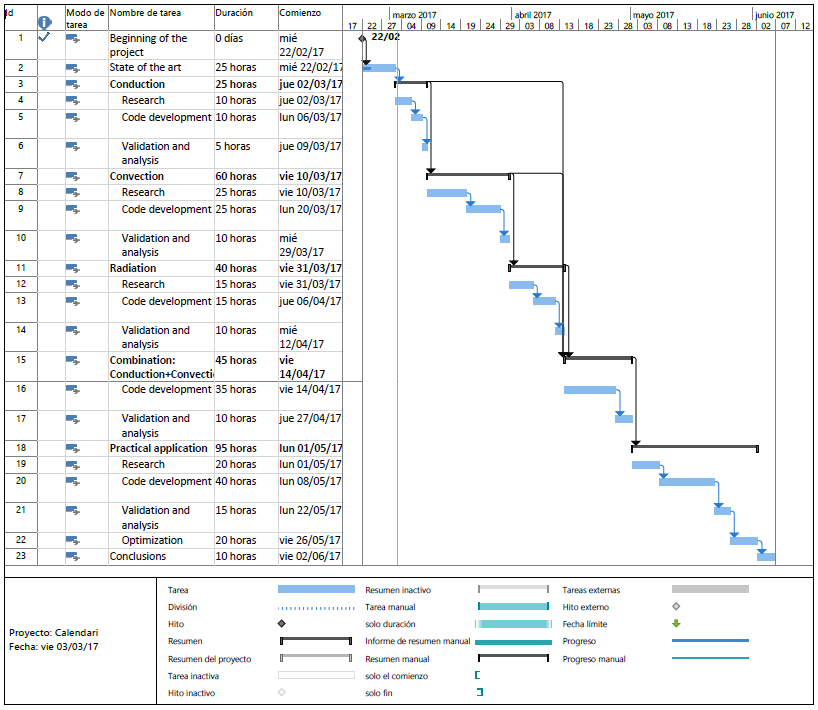
\includegraphics[scale=0.7]{Gantt}
\caption{Gantt Chart}
\end{figure}

\end{document}